%!TEX root = ../phd-thesis-lei-ma.tex
%!TeX spellcheck = en-US


\chapter{\label{chap:basics}Neutrino Oscillations in Vacuum}

Because the flavor eigenstates of the neutrino are not the same as its propagation eigenstates, it can change flavor while it propagates. To understand its flavor oscillation in vacuum, I will use the two-flavor scenario as an example\footnote{In most physical problems, two-neutrino-flavor scenario is a good approximation. The mass splits between the three mass eigenstates are so different that the corresponding oscillations occur on very diferent length scales. On the right length scale, the two-flavor scenario captures the significant features of the neutrino oscillations of the corresponding mass split.}. I will also explain how to visualize neutrino oscillations using the flavor-isospin picture.

Before working out the math, I can estimate the frequency of the oscillations of the neutrino between its flavors. In the natural units, frequency has the same dimension as energy (see Appendix~\ref{chap:app-sec:conventions-subsec:units}). Consider an electron neutrino with moment $p$ which is a superposition of the two mass eigenstates $\ket{\nu_i}$ ($i=1,2$) with masses $m_i$ respectively. Since the neutrino masses are small, I can Taylor expand the energy of each mass eigenstate in terms of the corresponding mass:
\begin{align}
E_i^{(v)} & = \sqrt{m_i^2 + p^2 } \nonumber\\
& = p \sqrt{\frac{m_i^2}{p^2} + 1} \nonumber\\
& \approx p + \frac{1}{2} \frac{m_i^2}{p},
\label{chap:basics-section:neutrinos-eqn:energy-taylor}
\end{align}
The constant energy term in the above equation produces a global phase to the flavor wave function which does not affect neutrino flavor oscillations. The characteristic energy scale in the problem is the difference of energies between the two mass eigenstates,
\begin{equation}
    \omega_{\mathrm v} =  \frac{m_2^2-m_1^2}{2E} = \frac{\delta m^2}{2E},
    \label{chap:basics-section:neutrinos-eqn:qualitative-method-frequency}
\end{equation}
which turns out to be the vacuum oscillation frequency. Here $E=p$ is approximately the energy of the neutrino.

To work out the exact solutions, I will utilize the Schr\"{o}dinger equation. The wave function in flavor basis $\Psi^{(\ff)}$ is related to the wave function in mass basis $\Psi^{(\vv)}$ through a unitary mixing matrix $\mathbf U$,
\begin{equation}
\Psi^{(\mathrm f)} = \mathbf{U}\Psi^{(\mathrm v)},
\label{chap:vacuum-eqn:wavefunction}
\end{equation}
where the upper indice ${}^{(v)}$ and ${}^{(f)}$ are used to denote the bases. The mixing matrix can be expressed using vacuum mixing angle $\theta_{\vv}$
\begin{equation}
\mathbf{U} = \begin{pmatrix} \cos\theta_\vv & \sin \theta_\vv \\ -\sin \theta_\vv & \cos \theta_\vv \end{pmatrix}.
\end{equation}
In vacuum mass basis, the neutrino has a free propagation Hamiltonian which is given by
\begin{equation}
\mathbf H^{(\vv)} = \begin{pmatrix} E_1 & 0 \\
0 & E_2
\end{pmatrix}.
\end{equation}
To the first order, the Hamiltonian becomes
\begin{align}
\mathbf H^{(\vv)} &= \frac{1}{2E} \begin{pmatrix}
m_1^2 & 0 \\
0 & m_2^2
\end{pmatrix} + E \mathbf{I} \nonumber \\
& =  \frac{1}{4E} \begin{pmatrix}
 - \delta m^2 & 0 \\
0 & \delta m^2
\end{pmatrix}  + \left(\frac{m_2^2 + m_1^2}{4E}  + E \right) \mathbf{I}.
\end{align}
Because a multiple of the identity matrix only gives an global phase to the neutrino flavor wave function, I will neglect it from now on:
\begin{equation}
\mathbf H^{(v)} =  \frac{\delta m^2}{4E} \begin{pmatrix}
-1 & 0 \\
0 & 1
\end{pmatrix} = -\frac{\delta m^2}{4E} \sigma_3 = -\frac{\omega_{v}}{2}\sigma_3.
\end{equation}
The Schr\"{o}dinger equation has a simple solution in mass basis,
\begin{equation}
\Psi^{(v)}(t) = \begin{pmatrix}
c_1(0) e^{i \omega_v t/2 } \\
c_2(0) e^{ -i\omega_v t/2 }
\end{pmatrix}.
\end{equation}
% where the initial condition is
% \begin{equation}
% \Psi_v^{(v)}(0) = \begin{pmatrix}
% c_1(0) \\
% c_2(0)
% \end{pmatrix}.
% \end{equation}
Using Eqn.~\ref{chap:vacuum-eqn:wavefunction}, I obtain the wave function at anytime is related to wave function in mass basis,
\begin{align}
\Psi^{(f)}(t) &= \mathbf{U}\Psi^{(v)}(t) \\
& = \begin{pmatrix} \cos\theta_v & \sin \theta_v \\ -\sin \theta_v & \cos \theta_v \end{pmatrix} \begin{pmatrix} c_1(0) e^{i\omega_v t/2 } \\
c_2(0) e^{ -i\omega_v t/2 }    \end{pmatrix} .
\label{chap:vacuum-eqn:wavefuncion-time}
\end{align}

Alternatively, I can also determine the Hamiltonian in flavor basis first, which is
%then solve the Sch\"{o}dinger equation. I will not show the steps here, however, the Hamiltonian in flavor basis is presented for future use,
\begin{equation}
\mathbf H^{(\ff)} = U H^{(\vv)} U^\dagger = -\frac{\omega_v}{2}\cos 2\theta_v \sigma_3 + \frac{\omega_v}{2} \sin 2\theta_v \sigma_1.
    \label{chap:basics-sec:vacuum-osc-eqn:hamiltonian-vacuum}
\end{equation}
By solving the Schr\"{o}dinger equation, I will obtain the same wave function as in Eqn.~\ref{chap:vacuum-eqn:wavefuncion-time}.

%In many astrophysical neutrino sources such as the solar core, electron neutrinos are the most abundant. Thus the initial condition is usually assumed to be electron flavor in the calculation which leads to the survival probability of electron flavor
The probability for an electron flavor neutrino at time $t$ is
\begin{equation}
P(\nu_e,t) = 1-\sin^2(2\theta_v)\sin^2\left( \frac{\omega_v t}{2} \right).
\end{equation}
Since the neutrino travels with approximately the speed of light, the electron neutrino survival probability at distance $L$ from the source is
\begin{equation}
P(\nu_e,L) =  1-\sin^2(2\theta_\vv)\sin^2\left( \frac{\omega_\vv}{2} L \right).
\end{equation}
An important parameter in vacuum oscillations is the oscillation length of the neutrino flavor conversion, $1/\omega_v$. This confirms our qualitative method result in Eqn.~\ref{chap:basics-section:neutrinos-eqn:qualitative-method-frequency}. I have plotted this result in Fig.~\ref{chap:basics-section:neutrinos-fig:vacuum-2-flavor-osc} which clearly shows the oscillatory behavior. The oscillation length is determined by the characteristic energy scale $\omega_v$, while the oscillation amplitude is determined by $\sin^2(2\theta_v)$.

\begin{figure}
    \centering
    \includegraphics[width=\textwidth]{chapters/assets/basics/neutrino-vaccum-osc-2-flavor.pdf}
    \caption{The electron flavor neutrino survival probability in vacuum oscillations as a function of distance $L$ which is measure in terms of vacuum oscillation $\omega_\vv$. The mixing angle is given by $\sin^2\theta_\vv=0.30 \approx \sin^2 \theta_{12}$.}
    \label{chap:basics-section:neutrinos-fig:vacuum-2-flavor-osc}
\end{figure}



\begin{figure}
	\centering
	\begin{subfigure}[t]{0.48\textwidth}
		\centering
		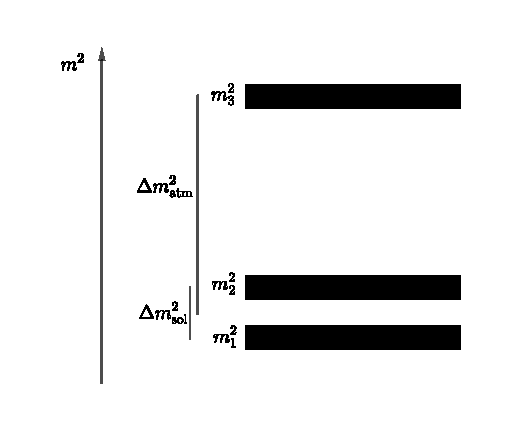
\includegraphics[width=\textwidth]{chapters/assets/basics/masses-nh}
		\caption{Normal hierarchy: the third mass is heavier than the first two.}
    \label{chap:basics-sec:flavor-isospin-pic-fig:masses-nh}
	\end{subfigure}
	\quad
	\begin{subfigure}[t]{0.48\textwidth}
		\centering
		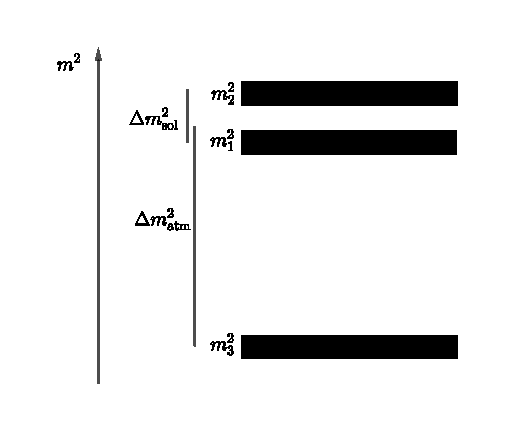
\includegraphics[width=\textwidth]{chapters/assets/basics/masses-ih}
		\caption{Inverted hierarchy: the third mass is smaller than the first two.}
    \label{chap:basics-sec:flavor-isospin-pic-fig:masses-ih}
	\end{subfigure}
	\caption{The order of the three neutrino masses. The difference between the first two masses is responsible for solar neutrino oscillations and the difference between the third mass and the first two is responsible for atmospheric neutrino oscillations.}
    \label{chap:basics-sec:flavor-isospin-pic-fig:masses}
\end{figure}

\begin{figure}
    \centering
    \includegraphics[width=\textwidth]{chapters/assets/basics/vacuum-oscillations-3-flavor.pdf}
    \caption{The probabilities for a $1MeV$ neutrino, which is in the electron flavor initially, in different flavors as functions of the distance. Neutrino vacuum oscillations with three flavors. The solid lines represent the normal hierarchy and the dashed lines represent the inverted hierarchy. The mixing angles are $\sin^2\theta_{12}=0.30$, $\sin^2\theta_{13}=0.023$, and $\sin^2\theta_{23}=0.41$, respectively, and the mass differences are $\delta m_{21}^2 = 7.9\times 10^{-5}\mathrm{eV^2}$ and $\delta m^2_{23}=2.7\times 10^{-3}\mathrm{eV^2}$.}
    \label{chap:basics-section:neutrinos-fig:vacuum-3-flavor-osc}
\end{figure}


In nature, there are three neutrino flavors and, correspondingly, three neutrino mass eigenstates, which are shown in Fig.~\ref{chap:basics-sec:flavor-isospin-pic-fig:masses}. Because there are two different characteristic energy scales, $\omega_{v,21}=\delta m_{21}^2/2E$ and $\omega_{v,32}=\delta m_{31}^2/2E$, two oscillation periods should occur, as shown in Fig.~\ref{chap:basics-section:neutrinos-fig:vacuum-3-flavor-osc}. The fast oscillations are determined by the larger energy scale, $\omega_{v,32}$, while the slow oscillations are determined by the smaller one $\omega_{v,21}$. For the inverted neutrino mass hierarchy (with $m_3 < m_1 < m_2$), the oscillation frequencies are the same as in the normal mass hierarchy (with $m_3>m_2>m_1$) since they have the same characteristic energy scales. However, they will develop different phases in oscillations.



\section{\label{chap:basics-sec:flavor-isospin-pic}Flavor Isospin Picture of Neutrino Oscillations}


\begin{figure}
    \centering
    \vspace*{-10pt}
    \includegraphics[width=\textwidth]{chapters/assets/basics/flavor-isospin-illus}
    \caption{In the flavor isospin picture, a flavor isospin pointing upward indicates that the neutrinos are in electron flavor, while the downward direction indicates the other flavor, such as the muon flavor.}
    \label{chap:basics-sec:flavor-isospin-pic-fig:flavor-isospin-illus}
\end{figure}

In principle, the oscillations in two flavor scenario are consequences of the Hamiltonian in this two-level quantum system. It is known that two-level quantum systems are visualized using the Bloch sphere. In the realm of neutrino physics, flavor isospin was introduced for such visualizations~\cite{Duan2006b}. The Hamiltonian for neutrino oscillations in vacuum (Eqn.~\ref{chap:basics-sec:vacuum-osc-eqn:hamiltonian-vacuum}) and in matter (Eqn.~\ref{chap:basics-sec:msw-eqn:hamiltonian-matter-effect}) can be reformulated into vector forms.

We start with the vector form of Hamiltonian for vacuum oscillations. Mathematically speaking, we will cast every two by two matrix into the quaternian basis,
\begin{equation}
    H^{(f)} = - \frac{\vec{\sigma} }{2}\cdot \vec H.
\end{equation}
Meanwhile, the state of neutrinos is represented by the flavor isospin, which is defined as
\begin{equation}
    \vec s = \Psi^{\dagger} \frac{\vec{\sigma} }{2} \Psi.
\end{equation}
As shown in Fig.~\ref{chap:basics-sec:flavor-isospin-pic-fig:flavor-isospin-illus}, the directions of the flavor isospin tell us the flavor content of the neutrino. We choose the direction of the third axis in flavor isospin space to point upward, so that a flavor isospin pointing upward indicates electron flavor by definition. In the flavor isospin formalism, the electron flavor survival probability is related to the third component of the flavor isospin,
\begin{equation*}
P = \frac{1}{2} + s_3.
\end{equation*}
Correspondingly, the equation of motion becomes precession around the Hamiltonian,
\begin{equation}
\dot{\vec s} = \vec s \times \vec H.
\label{chap:basics-sec:flavor-isospin-pic-eqn:eom-precession}
\end{equation}
The precession corresponds to periodic oscillations between flavors.

\begin{figure}
    \centering
    \vspace*{-20pt}
    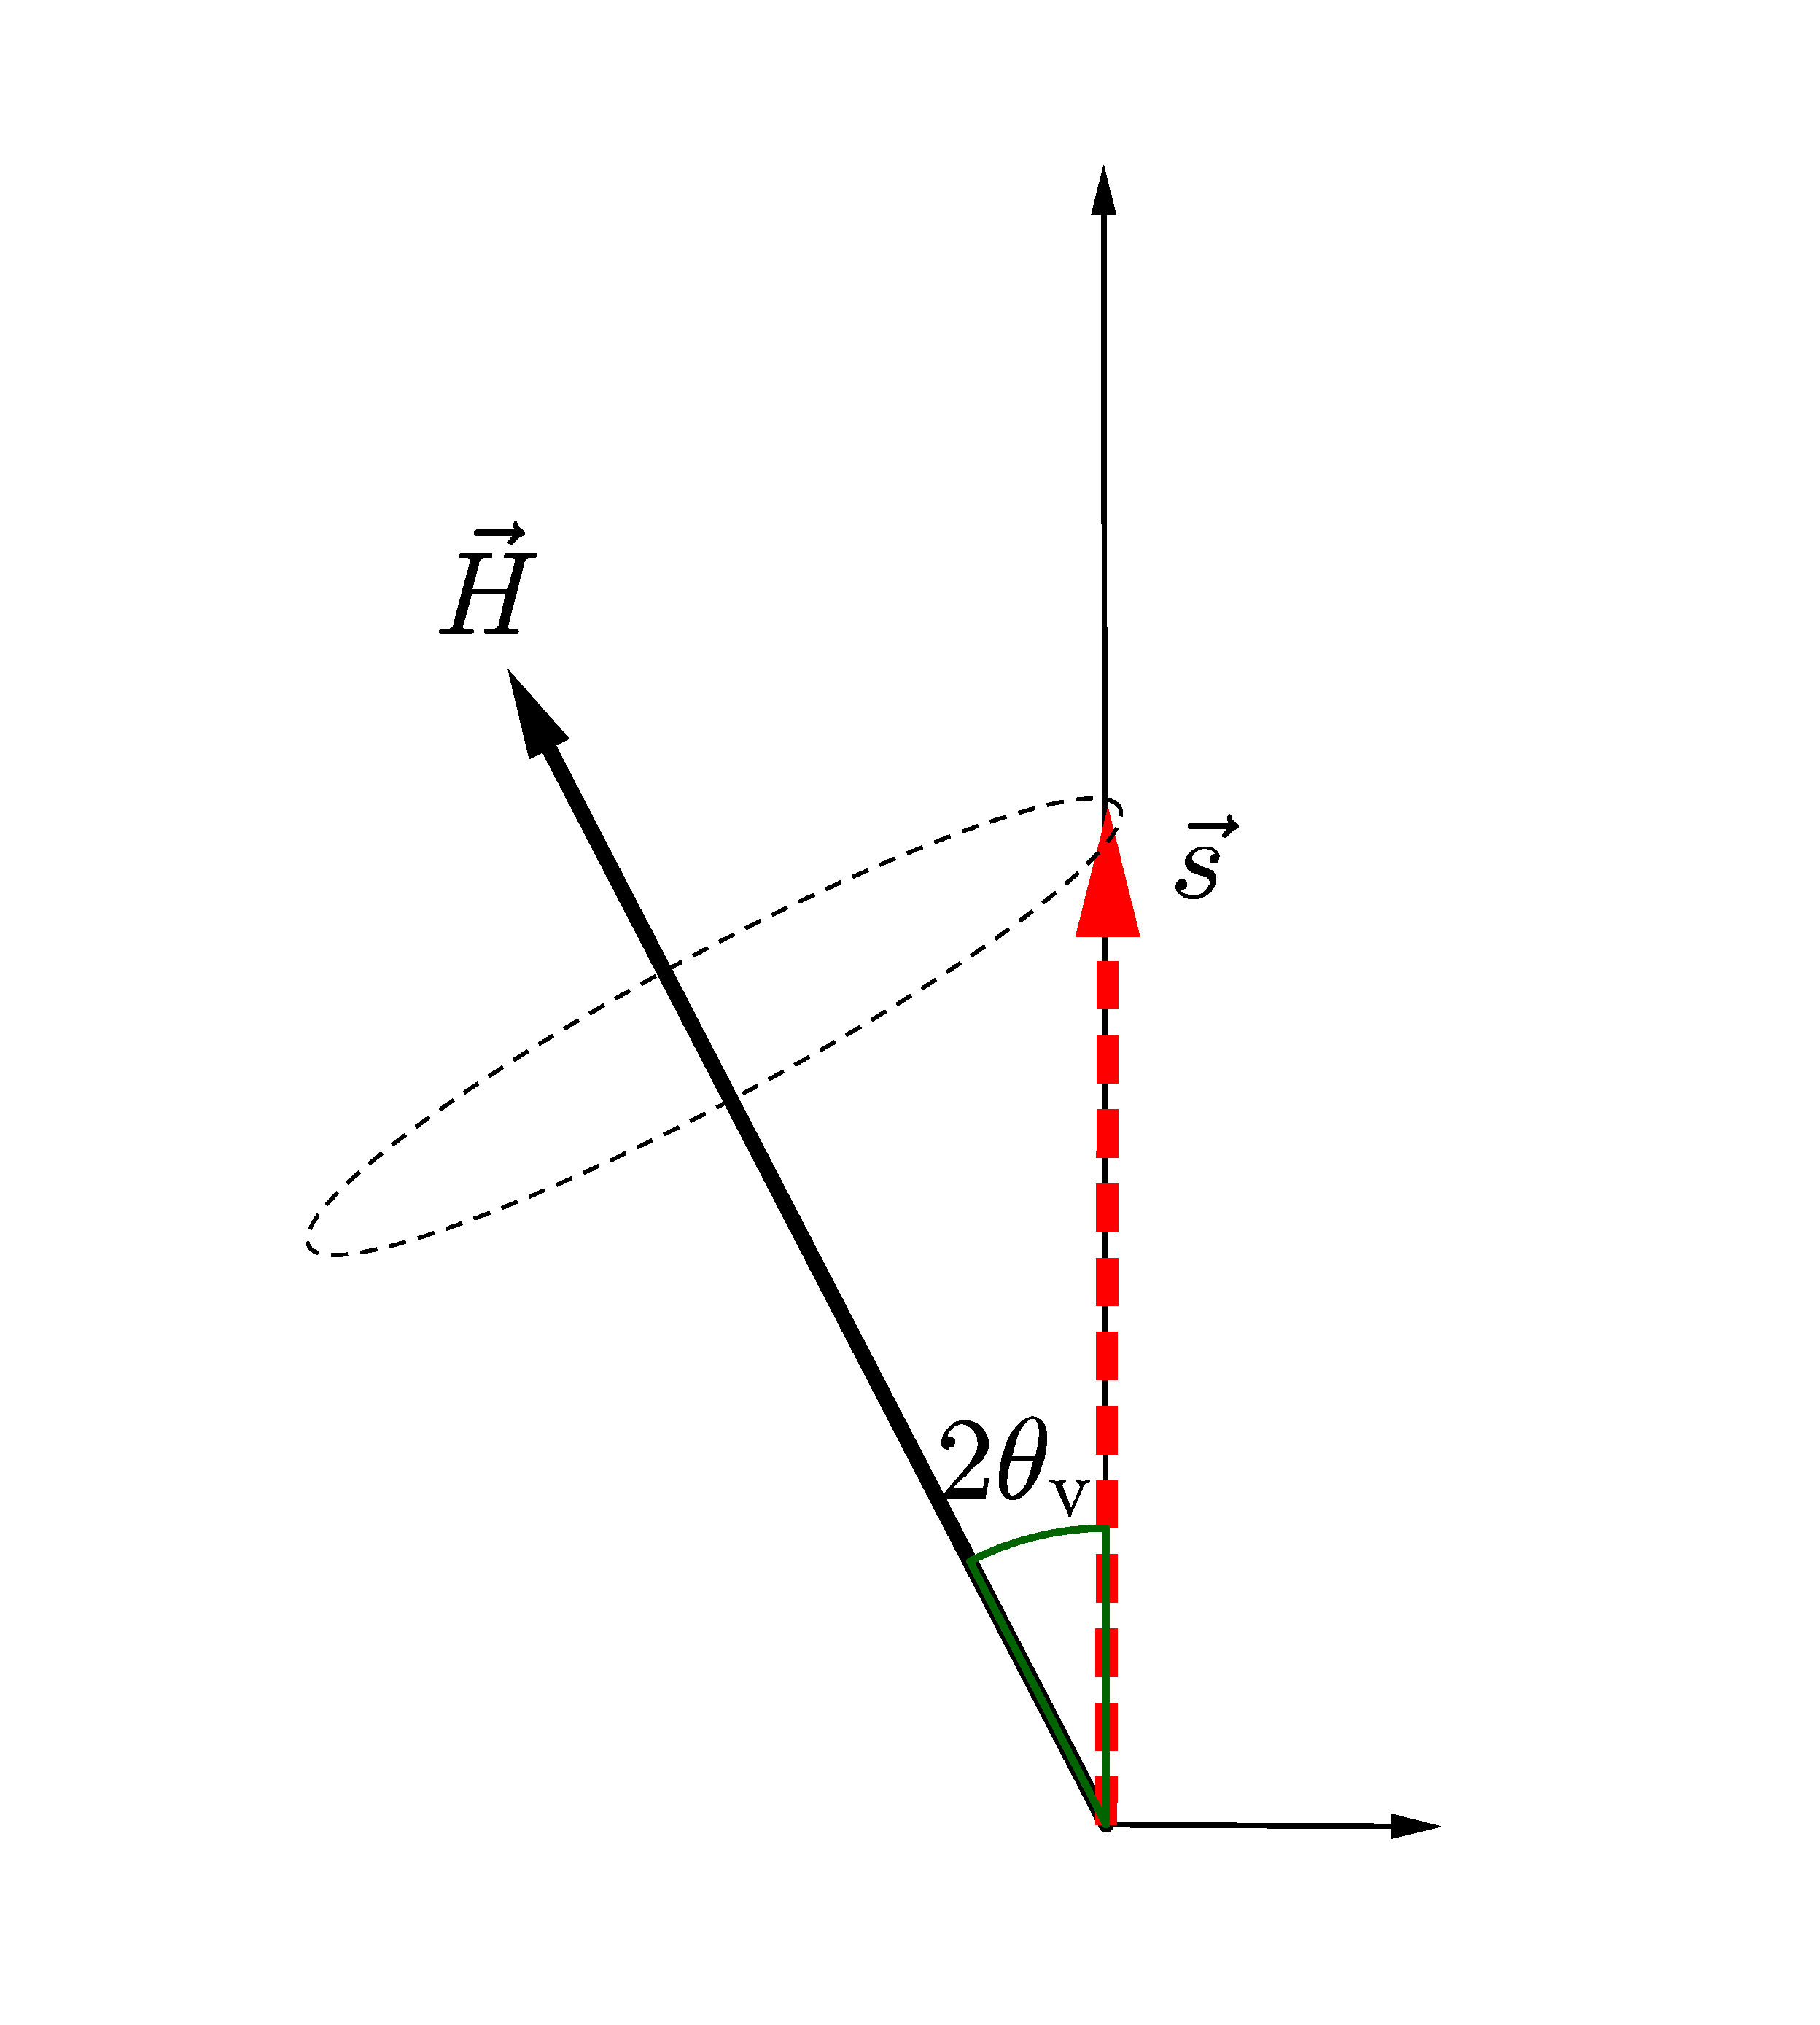
\includegraphics[width=0.6\textwidth]{chapters/assets/basics/flavor-isospin-vac-osc}
    \caption{Vacuum oscillations in flavor isospin picture. Neutrinos starting with electron flavor will follow a precession pattern around the static "Hamiltonian vector" $\vec H$, thus periodic flavor oscillations.}
    \label{chap:basics-sec:flavor-isospin-pic-fig:flavor-isospin-vac-osc}
\end{figure}


For example, in vacuum oscillations, vacuum oscillation Hamiltonian becomes
\begin{align*}
&\frac{\omega_{\mathrm v} }{2}\left( - \cos 2\theta_{\mathrm v } \sigma_3  + \sin 2\theta_{\mathrm{v}} \sigma_1 \right)
\to  \cos 2\theta_{\mathrm v}\begin{pmatrix}
0\\
0\\
\omega_{\mathrm v}
\end{pmatrix} -\sin 2\theta_{\mathrm v}\begin{pmatrix}
\omega_{\mathrm v}\\
0\\
0
\end{pmatrix},
\end{align*}
which is a vector of length $\omega_{\mathrm v}$ and tilted away from the third axis by the angle $2\theta_{\mathrm v}$. We assume neutrinos start with the electron flavor. Following the equation of motion Eqn.~\ref{chap:basics-sec:flavor-isospin-pic-eqn:eom-precession}, neutrinos precess around vector $\vec H$ that is tilted away from the vertical axis, as shown in Fig.~\ref{chap:basics-sec:flavor-isospin-pic-fig:flavor-isospin-vac-osc}. The oscillation frequency is trivially read out from the precession equation,
\begin{equation*}
    \omega_{\mathrm v} = \lvert \vec H_{\mathrm v} \rvert.
\end{equation*}





\section{Conclusion}

Vacuum neutrino oscillations is easily explained and calculated. However, it conveys the message of the nature of neutrino oscillations. Neutrinos are usually produced in flavor states since they are usually produced in weak interaction. The flavor states do not remain the same during the propagation since the flavor states are not the eigenstates of the propagation Hamiltonian. An extrapolation of this idea is that neutrinos might also oscillate for a constant linear potential. The Hamiltonian would be similar to vacuum Hamiltonian but with different values. One of such situations is neutrinos propagating through a region with constant matter density, which I will explain in Chapter~\ref{chap:matter}.
